\chapter{Introduzione}
Il mondo sta diventando sempre più interconnesso. Troviamo dispositivi connessi in quasi tutte le case e le reti informatiche sono il sistema nervoso delle organizzazioni aziendali e governative di tutto il mondo. Purtroppo per gli investigatori, Internet è stata progettata per la robustezza e la ridondanza, piuttosto che per la sicurezza e la tracciabilità. Questo aumenta la complessità e l'incertezza delle indagini digitali e rappresenta un'ardua sfida per gli informatici forensi. La digital forensics sta diventando sempre più importante con l'aumento del cybercrimine e di altri gravi reati informatici. Le prove digitali sono ovunque e svolgono un ruolo importante in quasi tutte le indagini penali come: piccoli reati, cybercrimine, crimine organizzato e anche il terrorismo. È quindi fondamentale che gli studenti di informatica e sicurezza acquisiscano una buona conoscenza della digital forensics, per poter agire come esperti in un contesto legale.

\section{Forensic Science}
\begin{figure}[h]
    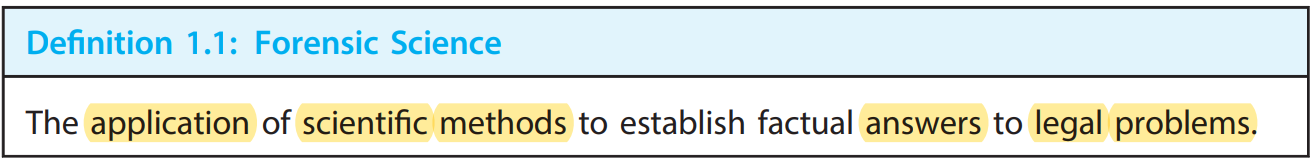
\includegraphics[width=\textwidth]{Capitolo 1/Figure/forensic-science-def.png}
\end{figure}

Le Forensic Science sono \textbf{l'applicazione di metodi scientifici che permettono di rispondere a problemi legali.}
Uno scienziato forense deve stabilire il cosa, il come, il chi e il quando; e per offrire queste risposte utilizza tool e strumenti relativi a scienze teoriche e applicate. Tuttavia non è sempre possibile ottenere la certezza totale per queste risposte e quindi uno scienziato forense a volte deve far ricorso a metodi statistici e probabilistici.

\subsection{Locard’s Exchange Principle}

\subsection{Ricostruzione del crimine}

\subsection{Investigazione}

\subsection{Evidence Dynamic}

\section{Digital Forensics}


    





